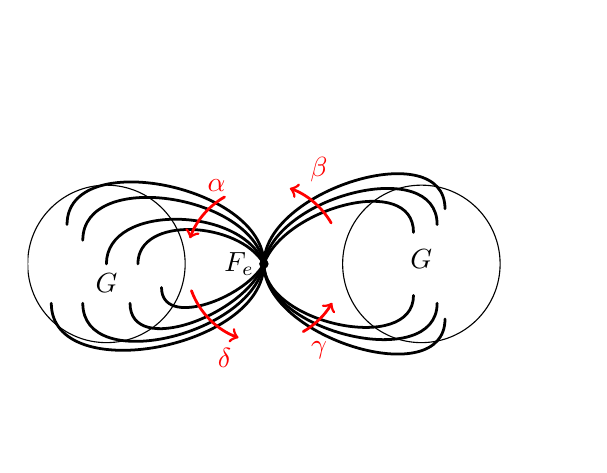
\begin{tikzpicture}[line cap=round,line join=round,x=1cm,y=1cm]
\clip(-1,-2.3) rectangle (6,3);

\draw (0,0) circle [radius=1cm];
\draw (4,0) circle [radius=1cm];
\draw (0,0) node[anchor=north] {$G$};
\draw (4,.3) node[anchor=north] {$G$};


\draw [line width=1pt] (2,0) to[out=90,in=90,looseness=1] (-.5,.5); % F0 -- F2
\draw [line width=1pt] (2,0) to[out=100,in=90,looseness=1] (-.3,.3); % F0 -- F2
\draw [line width=1pt] (2,0) to[out=110,in=90,looseness=1] (0,0); % F0 -- F2
\draw [line width=1pt] (2,0) to[out=120,in=90,looseness=1] (.4,0); % F0 -- F2


\draw [line width=1pt] (2,0) to[out=90,in=90,looseness=1] (4.3,.7); % F0 -- F3
\draw [line width=1pt] (2,0) to[out=80,in=90,looseness=1] (4.2,.5); % F0 -- F3
\draw [line width=1pt] (2,0) to[out=70,in=90,looseness=1] (3.9,.4); % F0 -- F3


\draw [line width=1pt] (2,0) to[out=-90,in=-90,looseness=1] (-.7,-.5); % F0 -- F2
\draw [line width=1pt] (2,0) to[out=-100,in=-90,looseness=1] (-.3,-.5); % F0 -- F2
\draw [line width=1pt] (2,0) to[out=-110,in=-90,looseness=1] (.3,-.5); % F0 -- F2
\draw [line width=1pt] (2,0) to[out=-120,in=-90,looseness=1] (.7,-.3); % F0 -- F2

\draw [line width=1pt] (2,0) to[out=-90,in=-90,looseness=1] (4.3,-.7); % F0 -- F3
\draw [line width=1pt] (2,0) to[out=-90,in=-90,looseness=1] (4.2,-.5); % F0 -- F3
\draw [line width=1pt] (2,0) to[out=-90,in=-90,looseness=1] (3.9,-.4); % F0 -- F3

\draw (2,0) node[anchor=east] {$F_e$};
\draw [fill=black] (2,0) circle (1.5pt);

% Arcos
%\draw (2,0) circle [radius=1cm];

\draw[red,line width=1pt,<-] (2.33,.96) arc (70:30:1);
\draw (2.7,1.2) node[red] {$\beta$};

\draw[red,line width=1pt,->] (1.5,.85) arc (120:160:1);
\draw (1.4,1) node[red] {$\alpha$};

\draw[red,line width=1pt,->] (1.08,-.34) arc (200:250:1);
\draw (1.5,-1.2) node[red] {$\delta$};

\draw[red,line width=1pt,->] (2.5,-.86) arc (-60:-30:1);
\draw (2.7,-1.1) node[red] {$\gamma$};
\end{tikzpicture}
